\documentclass[a4paper]{article} % a4paper option recommended
\usepackage[english]{babel}
\usepackage{uureport}
\usepackage{cite}
\usepackage{hyperref}
\usepackage{pgfplots}
\usepackage{float}
\bibliographystyle{alpha}

\title{Diplomacy}
\type{Report}
\course{Games \& Agents}

\author{A. Berland, B. Reigersberg, E. Koens, \\J. de Groot, K. van Katwijk, T. de Goey}

\begin{document}
\maketitle
\tableofcontents
\newpage

\section{Introduction}
Diplomacy is an online multiplayer game based on the board game invented in 1954 by Allan B. Calhamer. The online version of the game has 137966 subscribed players, it can however be played by bots as well. A few bots have already been implemented, so far the best bot on the market is Albert. All these bots lack one common property, which is the ability to asses the other players. Therefore we tried to implement an Artificial Intelligent bot for this game, which is able to comprehend the actions of other bots and players. Our bot can deduce the best possible moves which are based on his own ideas and knowledge, he will also concern his current belief on the other player or bot. We made quite some progress and we will elaborate on our development of this bot in this paper.

\subsection{Diplomacy}
The online diplomacy game is based on the map of 1901 Europe, but can also be played on other maps. The map consists of three different nodes. These are divided in land provinces, coastal provinces and sea nodes.
\\The goal of the game is to be the first to hold more than half of the supply centers. Supply centers can be divided in two types, Home Supply Centers and other Supply Centers (there is no actual difference in the game it self but we made the difference for the weight \& gains system). All Supply Centers sustain the military units, however only Home Supply Centers can build new units. In order to build new units a player has to own more Supply Centers than units this is done in the Build phase (Winter).
\\There are five phases in Diplomacy, as stated earlier there is the Build phase, which is called Winter in game. There are two Order phases (Summer and Fall) in which the player decides where to move his available units. After each order phase there is a retreat phase (Spring and Autumn). In the retreat phase any attacked units are forced to retreat. If there is no possible place to retreat to the unit needs to be disbanded (removed from the game).
\\The game revolves around two different type of units. On one side there is the Army unit type which moves on coastal and land provinces. The other unit type is the Fleet, this unit can move through coastal provinces and trough oceans. The Fleets can convoy Army units over the sea to other provinces. The armies all have the same power, so in order to take a province a player needs support moves.
\\The units have five types of moves. The first move is the HOLD move. With this move the unit stays on his current territory and therefore defend it.
Then there is the MOVE action, with it the unit moves from one province to an adjacent province.
Then there are two types of support moves, the SUPPORT HOLD, this is a support for the defending HOLD move. The SUPPORT HOLD gives the defending army an additional unit to defend with. And then there is the SUPPORT MOVE, which is basically the same but for attacking. The last move is the CONVOY move, for this move a player needs a fleet and an army. The fleet needs to be in the ocean. Then the army moves via the fleet over the ocean to the next province.
The CONVOY move can also be chained if mutiple fleets are adjacent, this is still seen as one move.


\section{Gain system}

In order for our AI to know where it should move it's units to, we make use of a gain system. For every province we calculate a gain value. This value signifies the importance of this province based on a variety of properties and heuristics. We weigh this gain with factors such as likeliness to succeed and whether we defect allies by moving to this province. 

\subsection{Gains}  

For each province the gain value signifies the importance of that province. To calculated the gain, we have selected a number of properties which we believe makes a province important (But can very easily be extended and adjusted). We divided these into four categories. 

\begin{itemize}
\item Supply gain
\item Defend gain
\item Counter gain
\item Kill gain
\end{itemize}

\subsubsection{Supply gain}

The supply gain is given to provinces which contain a supply center. In order to win the game one has to control more than half of all the supply centers. Also, the number of supply centers you control determines how much units you are allowed to have. Therefore, capturing supply centers is crucial to winning the game and these provinces are important and we give these a gain. There are however different types of supply centers we have to consider. 

Supply centers can be controlled by a power. If a supply center is not controlled by us (so either neutral or under control by any other power), we can potentially take over this supply center. We give these a gain $g_{supply}$. Supply centers we control have no real gain as we can not take them over again. However, in the case that there is nothing more important to do, we would prefer units to move to one of our supply centers as a means of defence. We therefore give a small symbolic gain $g_{ourSupply}$ to supply centers we own. 

Some supply centers are home supply centers. These are home to a specific power and a power can only build new units on his home supply centers. Additional to the importance of normal supply centers, capturing a home supply center from a power effectively disables this power from building new units there. Therefore we give these a different (higher) gain $g_{home}$. We only do this when this home supply center is under control by the corresponding power. If this is not the case, then this power is already blocked from building units there and there is no additional gain from taking this. In this case we treat is as a normal supply center and give gain $g_{supply}$.

Following this rule, our own home supply centers are also very important. As with normal supply centers, if we control them they get a small gain $g_{ourHome}$. However, if a home supply center is under control by another power it is very important to get it back in order to build new units. In this we assign a very high gain $g_{takenHome}$. 

\subsubsection{Defend gain}

Without defending the supply centers we already control, they will just as easy be taken back from us. The defend gain is therefore given to supply centers we control and are under threat. In order to do this we first have to quantify threat. We calculate the threat by a weighted sum of the first and second order enemies from the same power (e.g. the enemies one tile away and the enemies two tiles away respectively). 

$$threat = max_{threat_j}\{ threat_j : C_1 \sum_{i} e^{1}_{ij} + C_2 \sum_{i} e^{2}_{ij}\}$$

We have chosen to give the supply center a defend gain $g_{defend}$ if $threat > \varepsilon_{threat}$. As we belief that defending home supply centers is more important these get a different gain $g_{defendHome}$. 

\subsubsection{Counter gain}
Using only the aforementioned gains, we perceived that units on threatened home supply centers displaying  ``camping'' behaviour. The unit keeps defending the home supply center from a neighbouring enemy whereas the neighbouring is interested in the home supply center and hence does not move away. We therefore introduced a high counter gain $g_{counter}$, to provinces adjacent to a home supply center and containing an enemy unit. This way, instead of endlessly holding the home supply center, units will start to make offensive moves against adjacent enemies driving the threat away instead of waiting for it to go.        

\subsubsection{Kill gain}
Another thing we also witnessed by watching our AI play is that very often units of a power are on the far side of the map - far from any support. This units are often left unattended as a single unit is not considered a threat. We therefore introduced a kill gain $g_{kill}$. This is a very high gain for a province containing a lonely enemy unit (no other enemy units as close as two tiles away), and this unit has limited provinces $< \varepsilon_{kill}$ to retreat to - likely causing it to disband when attacked. 
Another issue solved by this, is that very often the last living unit of a power is left unattended and sometimes even regains considerable power. 

\subsection{Smoothing gains}


\subsubsection{Gain values}

We chose this gain because blablabla. This one should then be higher because bla. Therefore bla. Blip bloop blababliebloopie. 

\begin{figure}[H]
\centering
\begin{tabular}{| l | c |}
  \hline            
  {\bf Gain} & {\bf Value}\\
  {Supply Gains} &  \\
  $g_{supply}$ & 3.0 \\
  $g_{ourSupply}$ & 0.25 \\
  $g_{home}$ & 3.2 \\
  $g_{ourHome}$ & 0.3 \\
  $g_{takenHome}$ & 5.0 \\
  {Defend gains} &  \\
  $g_{defend}$ &  3.0 \\
  $g_{defendHome}$ & 3.2 \\
  {Counter gain} & \\
  $g_{counter}$ & 5.5 \\
  {Kill gain} & \\
  $g_{kill}$ & 5.0 \\
  \hline  
\end{tabular}
\caption{Values choses for the various gain variables}
\end{figure}


    % public static float c_smooth = 0.25f;
    % public static float c_threat = 1.0f;
    
    % public static float c_shared = 0.0f;
    % //public static float risk = 1.0f; 
    % //public static float sharedRisk = 1.0f;
    % public static float defence = 1.0f; 

    % public static float takeOverRisk = 0.5f;

    % public static float c_normalNotOurs = 3.0f; 
    % public static float c_homeNotOurs = 3.2f; 

    % public static float c_normalOurs = 0.25f; 
    % public static float c_homeOurs = 0.30f; 

    % public static float c_normalOursThreat = 3.0f; 
    % public static float c_homeOursThreat = 3.2f; 

    % public static float c_homeOursTaken = 5.0f; 

    % public static float c_threatThreshold = 1.10f; 

    % public static float c_counter = 5.5f; 

    % public static float c_kill = 5.0f; 

    % public static float attackThreshold = 3.0f; 



\subsection{Threat}

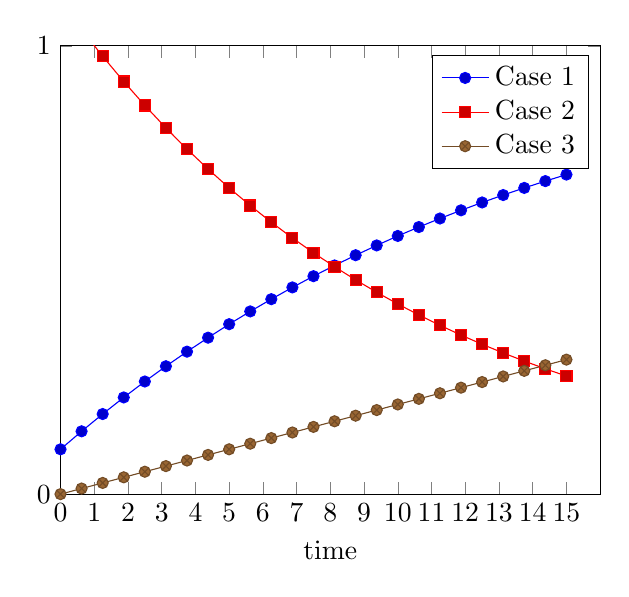
\begin{tikzpicture}
  \begin{axis}[ 
    xlabel= time,
    ylabel={},
    xtick = {0,1,2,3,4,5,6,7,8,9,10,11,12,13,14,15},
    ytick = {0,1},
    xmin = 0,
    ymin = 0,
    xmax = 16,
    ymax = 1,
    domain = 0:15
  ] 
    \addplot {1-((1.1^(-x))*(0.9+0.02*x))};
    \addplot {(1.1^(1-x))};
    \addplot {0.02*x};
    \legend{Case 1,Case 2, Case 3};
  \end{axis}
\end{tikzpicture}

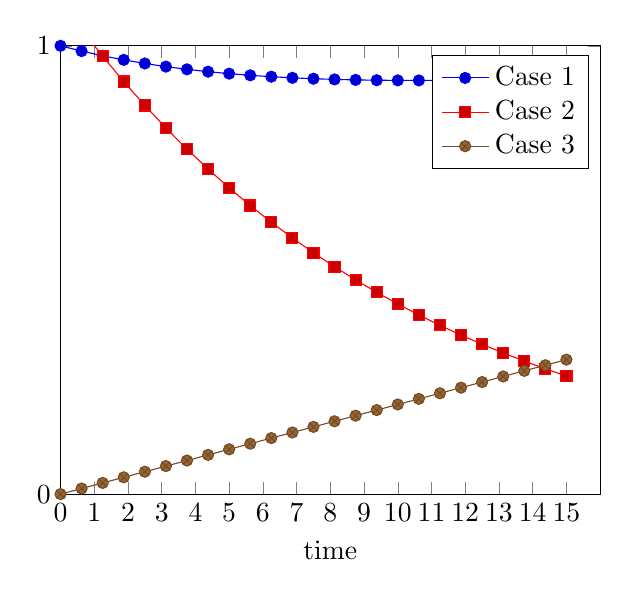
\begin{tikzpicture}
  \begin{axis}[ 
    xlabel= time,
    ylabel={},
    xtick = {0,1,2,3,4,5,6,7,8,9,10,11,12,13,14,15},
    ytick = {0,1},
    xmin = 0,
    ymin = 0,
    xmax = 16,
    ymax = 1,
    domain = 0:15
  ] 
    \addplot {1-((1.1^(-x))*(0.0+0.02*x))};
    \addplot {(1.1^(1-x))};
    \addplot {0.02*x};
    \legend{Case 1,Case 2, Case 3};
  \end{axis}
\end{tikzpicture}


% \begin{thebibliography}{1}

%   \bibitem{notes} Pacheco, J.M., Santos, F.C., Souza, M.O. and Skyrms, B., {\em Evolutionary dynamics of collective action in N-person stag hunt dilemmas}  2009.

%   \bibitem{impj}  da Costa Ferreira, A.F., {\em DipBlue: a Diplomacy Agent with Strategic and Trust Reasoning} For Jury Evaluation.

% \end{thebibliography}

\bibliography{references}{}

\end{document}
